\chapter{Introduction to Arduino}
\label{ch:arduino-uno}
Arduino is it one of the most widely used micro-controller to develop various DIY projects. The low cost and easy to deploy has given rise to various IoT and embedded projects. Arduino is an open source electronics platform based on easy-to-use hardware and software. Usually the term “Arduino” can be used to refer the following.
\begin{itemize}
    \item Open Source Electronics Platform : Free to design and implement various units, easy availability and high customization. 
    \item Arduino IDE [ Integrated Development Environment ] : A software to program Arduino boards.
    \item Online Arduino Community : Fast growing community who maintains and supports Arduino Developments.

\end{itemize}

\url{https://github.com/arduino/} \hspace{0.5cm} \url{https://www.arduino.cc/}

\par The Arduino project was started in 2005 as a program for students at the Interaction Design Institute Ivrea in Ivrea, Italy , aiming to provide a low-cost and easy way for novices and professionals to create devices that interact with their environment using sensors and actuators. The name Arduino comes from a bar in Ivrea, Italy, where some of the founders of the project used to meet. The ease at which various units can be attached gained Arduino its popularity. Anyone can start with programming and robotics by just following the step by step instructions of a kit, or sharing ideas online with other members of the Arduino community.

Following are few of the key points of Arduino :

\begin{itemize}
    \item Easy to use and expensive
    \item Cross-platform and open source
    \item Simple and clear programming
    \item  Extensible software/hardware
\end{itemize}

\begin{marginfigure}
    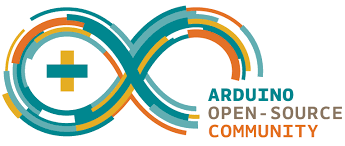
\includegraphics[width=2in]{Chapters/images/Arduino_opensource.png}
\end{marginfigure}    

\section{Comparing Arduino to its alternatives
}
Arduino is not the only board available to build custom projects and applications. Raspberry Pi, BeagleBone, Sharks Cove, Minnowboard MAX, Nanode, Waspmote or LittleBits are some of the most interesting alternatives to Arduino. Arduino and Raspberry Pi are the ones receiving the most attention within the community of software developers.

Raspberry Pi is a low cost Single Board Computer (SBC) developed by the British Raspberry Pi Foundation. They are used in places which require higher and faster calculations. They are boards with micro processors. Raspberry Pi acts as a mini computer with additional I/O connection pins along with Wi-Fi, Bluetooth and ability to connect to external devices via HDMI, USB ports etc.. It have a complete Operation System (Raszzberian) burned into a SD card. 

Arduino, on the other hand is a low cost System on Chip (SoC) board. They are used where complex information need not be analyzed. They are heavily used in Embedded systems and IoT. They are boards with micro controller that control other appliances. There are no Operating System burned into Arduino. Arduino simply uses machine code to execute instructions. The machine code are created by compiling programs written in high level languages like C, into an executable binary file.
\begin{figure}
\begin{multicols}{2}
    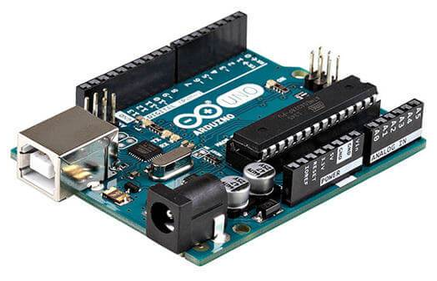
\includegraphics[width=2in]{Chapters/images/Arduino_uno.png}\par
    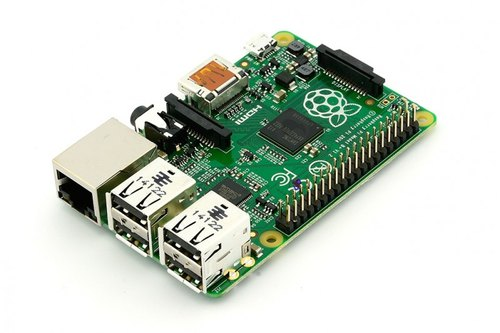
\includegraphics[width=2in]{Chapters/images/raspeberry_modelb.jpg}
\end{multicols}
\end{figure}